\documentclass{article}
\usepackage{graphicx}
\usepackage{titling}
\usepackage{pgfgantt}
\usepackage{pdflscape}
\usepackage{hyperref}
\usepackage{animate}
\usepackage{movie15}
\usepackage{array}
\usepackage{booktabs}
\usepackage{caption}
\usepackage{amsmath}

\renewcommand{\refname}{Kaynakça}
\pretitle{
  \begin{center}
  \LARGE\bfseries
  
\includegraphics[width=0.1\textwidth]{logo.png} 
  \vskip 1em
  }
  \posttitle{
  \end{center}
}
\title{Yapay Zeka ile Görüntü Gürültüsü Azaltma Projesi}
\author{İlyas Cemal Erginli}
\date{Mart 2024}

\begin{document}
\begin{titlepage}
    \maketitle
    \begin{center} 
        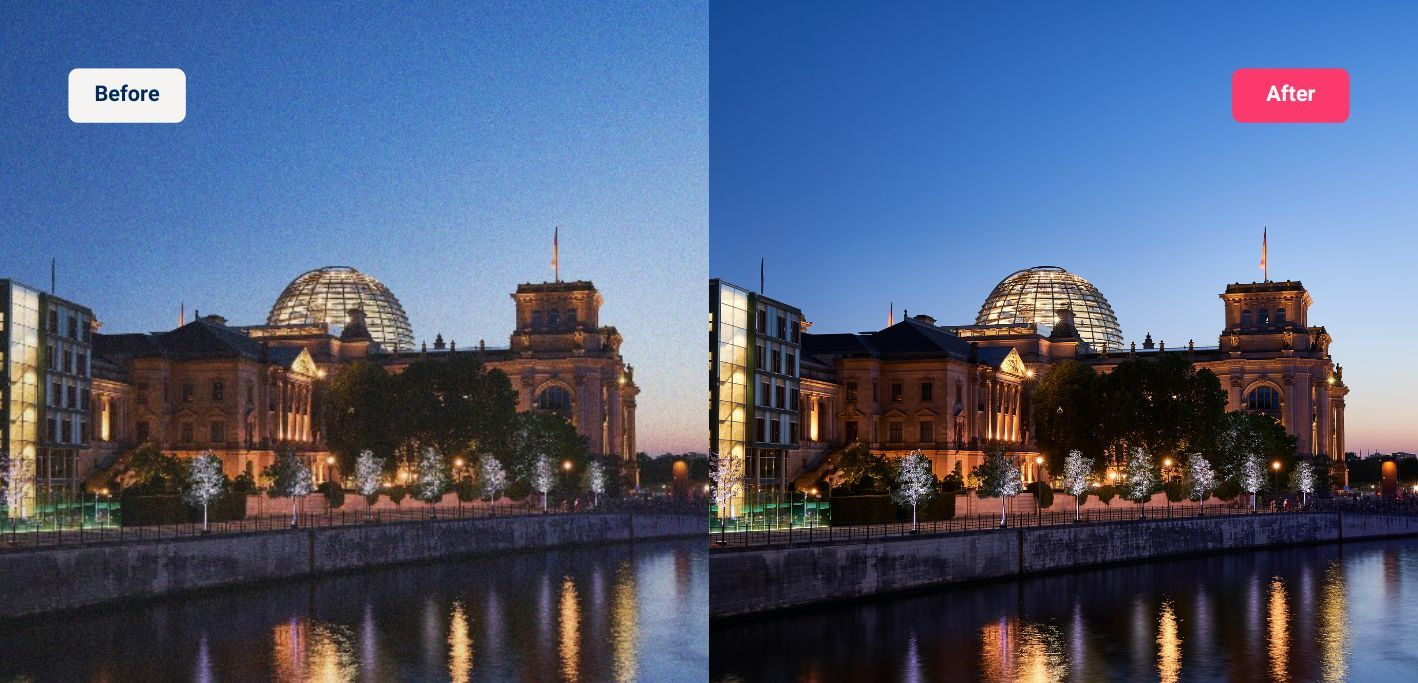
\includegraphics[width=0.8\textwidth]{imageAı.jpg}
    \end{center}
    \thispagestyle{empty}
    \vfill
    \rule{\textwidth}{0.5pt}
    \renewcommand{\abstractname}{Özet}
    \begin{abstract}
    \noindent Bu projenin amacı, gürültülü görüntülerdeki istenmeyen gürültüyü azaltarak veya ortadan kaldırarak daha net ve kaliteli görüntüler elde etmektir. Bu proje, çeşitli alanlarda (örneğin, tıbbi görüntüleme, fotoğrafçılık, video işleme) kullanılabilecek, gürültülü görüntülerin kullanışlılığını artırmayı hedefler. Yapay zeka modelleri, gürültülü görüntülerdeki desenleri ve yapıları tanıyarak gürültüyü azaltmak için öğrenilmiş bilgiyi kullanır. Bu proje, daha iyi görsel kalite ve daha doğru analiz sonuçları elde etmek için gürültülü görüntülerin iyileştirilmesine odaklanır.
    \end{abstract}
    \rule{\textwidth}{0.5pt}
    \vfill

\end{titlepage}
\newpage

\noindent \section{Giriş}
\rule{\textwidth}{0.5pt}\\[10pt]
Günümüzde, dijital görüntüleme teknolojileri hızla gelişmekte ve yaygın bir şekilde kullanılmaktadır. Ancak, bu teknolojilerin kullanımında sıkça karşılaşılan bir sorun da görüntülerin gürültülü olmasıdır. Gürültü, birçok faktörden kaynaklanabilir ve görüntülerin kalitesini düşürerek bilgi kaybına neden olabilir. Bu nedenle, görüntü gürültüsünün azaltılması, görüntüleme teknolojilerinin etkinliğini artırmak ve veri analizi süreçlerini iyileştirmek için önemli bir gerekliliktir. \\[10pt]

 \noindent Bu proje, yapay zeka tekniklerini kullanarak görüntü gürültüsünün azaltılmasını hedeflemektedir. Yapay zeka, özellikle derin öğrenme teknikleri, karmaşık veri yapılarını işleyebilme yetenekleriyle gürültü azaltma işlemlerinde etkili bir şekilde kullanılmaktadır. Bu proje kapsamında, gelişmiş yapay zeka algoritmaları ve derin öğrenme modelleri, gürültülü görüntülerin temizlenmesi için kullanılacak ve daha net ve kaliteli görüntüler elde edilmesi sağlanacaktır.\\[10pt]

\section{Literatür Çalışması}
\rule{\textwidth}{0.5pt}

 \noindent Bu makalede\cite{zhang2018ffdnet}, Hızlı ve etkili bir görüntü gürültü giderme yöntemi olan FFDNet, ayırt edici öğrenme yöntemlerinden farklı olarak geniş bir gürültü seviyesi aralığını tek bir ağla ele alabilir. Esnek bir yapıya sahip olan FFDNet, giriş olarak ayarlanabilir bir gürültü seviye haritası kullanarak mekansal olarak değişken gürültüyü de çıkarabilir. Ayrıca, örnekleme yapılmış alt görüntüler üzerinde çalışarak hızlı çıkarım hızı sağlar ve BM3D'e kıyasla daha hızlı sonuçlar elde eder. Yapılan deneyler, FFDNet'in etkili ve verimli olduğunu göstermiştir, bu da pratik gürültü giderme uygulamaları için cazip bir seçenek haline getirir.\\[10pt]

 \noindent Bu makalede\cite{yu2019deep}, Düşük seviye görüş araştırmalarında yaygın olarak incelenen özellik haritalarının indirme ve yükleme ölçeklendirme kullanılarak ağlar, verimli GPU bellek kullanımı ve geniş duyarlı alanları sağlama kapasiteleri nedeniyle incelenmiştir. Bu bağlamda, görüntü gürültü giderme için derin tekrarlayan indirme-yükleme evrişimli sinir ağı (DIDN) önerilmektedir. Bu ağ, özellik haritalarının çözünürlüğünü tekrar tekrar azaltıp artırır. Ağın temel yapısı, özgün olarak anlamsal segmentasyon için geliştirilen U-Net'ten esinlenmiştir. İndirme ve yükleme katmanları, görüntü gürültü giderme görevi için uyarlanmıştır. Geleneksel gürültü giderme ağları, tek seviyeli gürültüyle çalışması için eğitilmiştir veya alternatif olarak, tek bir modelle çoklu seviyeli gürültüyü ele almak için gürültü bilgisini giriş olarak kullanır. Bununla birlikte, ağımızın etkili bellek kullanımı, tek bir modelle gürültünün geniş bir aralığını işlemesini sağlar ve bu da gürültü bilgisi girişlerine ihtiyaç duymadan çoklu seviyeli gürültüyü ele almasını sağlar.\\[10pt]


\noindent
\section{Metadoloji}
\rule{\textwidth}{0.5pt}
Bu projede, Convolutional Neural Network (CNN) gibi derin öğrenme yöntemleri yanı sıra, temiz veri oluşturma için kullanılan autoencoder gibi unsupervised öğrenme teknikleri de kullanılacaktır. Autoencoder'lar, gürültülü görüntüyü giriş olarak alıp, gizli katmanlarda temiz görüntüyü oluşturarak gürültü azaltma sürecini gerçekleştirirler. Ayrıca, gürültülü görüntülerdeki istenmeyen özelliklerin tanımlanması için denetimli öğrenme yöntemleri de uygulanabilir. Bu yöntemlerde, gürültülü ve temiz görüntülerin eşleştirildiği bir eğitim veri seti kullanılarak, gürültülü görüntülerden temiz görüntülerin tahmini için öğrenme gerçekleştirilir.\\[10pt]

 \noindent Bu farklı yöntemlerin kombinasyonu, gürültü azaltma sürecindeki etkinliği artırabilir ve çeşitli gürültü tipleriyle başa çıkabilme kabiliyetini sağlayabilir. Autoencoder'lar, gürültülü verilerden temiz verilerin oluşturulmasında kullanılarak, CNN'lerin daha iyi performans göstermesine yardımcı olabilir. Denetimli öğrenme yöntemleri ise belirli gürültü tiplerine özgü özelliklerin tanımlanması ve gürültü azaltma işleminin hassaslaştırılması için önemli bir rol oynar. Bu yöntemlerin bir araya getirilmesi, daha güçlü ve esnek bir gürültü azaltma çözümü elde etmek için önemlidir.\\[5pt]


 \noindent Modeller:
\begin{enumerate}
    \item Autoencoder
    \item FFDNet(Feedforward Neural Network)
    \item DnCNN(Denoising Convolutional Neural Network)
    
\end{enumerate}

\newpage
\subsection{Aoutoencoders}

\noindent Aoutoencoderlar, görüntüler, vektörler, ses veya buna benzer bir tür giriş verisi alan ve önce orijinal giriş verilerini daha düşük bir boyuta sıkıştıran ve ardından verilerin bu daha düşük boyutlu temsilini kullanan bir tür yapay sinir ağıdır.
Eğitim süreci boyunca, kayıp fonksiyonu kullanılarak encoder ve decoder ağlarındaki parametreler ayarlanır. Bu ayarlamalar, encoder ve decoder'ın veriyi sıkıştırma ve tekrar oluşturma yeteneklerini geliştirir.\vspace{1 cm}

Mean Squared Error (MSE) 
\begin{equation}
    \frac{1}{n} \sum_{i=1}^{n} (x_{i} - \hat{x}_{i})^2
\end{equation}

Mean Absolute Error (MAE)
\begin{equation}
    \frac{1}{n} \sum_{i=1}^{n} |x_{i} - \hat{x}_{i}|
\end{equation}

\renewcommand{\figurename}{Şekil}

\begin{figure}[htbp]
     \centering
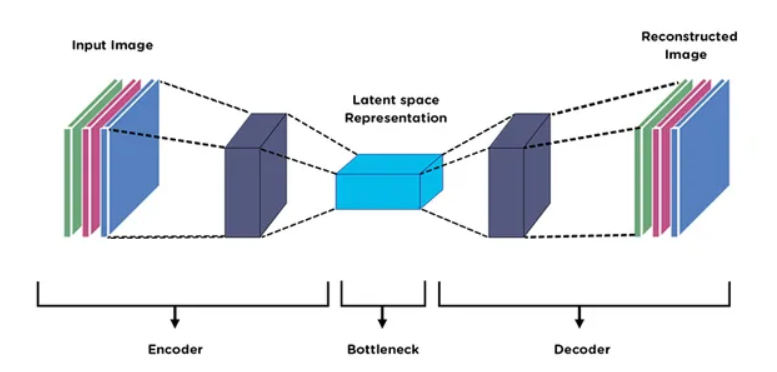
\includegraphics[angle=360,width=1.1\textwidth]{autoencoder.png}\centering 
  \caption{Aoutoencoder\cite{Autoencoder}}
  \label{fig:resim_etiketi}
\end{figure}

\newpage
\subsection{FFDNet}

\noindent Giriş görüntüsü alt görüntüler halinde yeniden şekillendirilir ve bunlar daha sonra bir gürültü seviyesi haritasıyla birlikte CNN’e girilir. Nihai çıktı, gürültüden arındırılmış alt görüntüler tarafından yeniden oluşturulur. Bu modelde de kayıp fonksiyonu kullanılır.
\vspace{1 cm}

Mean Squared Error (MSE) 
\begin{equation}
    \frac{1}{n} \sum_{i=1}^{n} (x_{i} - \hat{x}_{i})^2
\end{equation}

\renewcommand{\figurename}{Şekil}

\begin{figure}[htbp]
     \centering
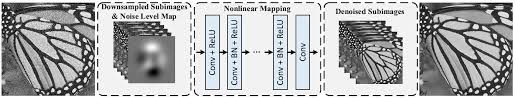
\includegraphics[angle=360,width=1.1\textwidth]{ffdnet.jpeg}\centering 
  \caption{FFDNet\cite{zhang2018ffdnet}}
  \label{fig:resim_etiketi}
\end{figure}

\subsection{DnCNN}

\noindent DnCNN, bir dizi evrişim katmanı, ReLU aktivasyon fonksiyonları ve gürültü azaltma amacıyla tasarlanmış özel bir eğitim kaybı fonksiyonunu içerir. Evrişim katmanları, görüntüdeki özellikleri çıkarmak ve öğrenmek için kullanılırken, ReLU aktivasyon fonksiyonları ağın doğrusallığı kırarak daha karmaşık özellikleri öğrenmesine yardımcı olur. Eğitim süreci boyunca, ağ gürültülü görüntüler ile temiz görüntüler arasındaki farkı minimize etmeyi öğrenir. Bu modelde de kayıp fonksiyonu kullanılır.\vspace{1 cm}

Mean Squared Error (MSE) 
\begin{equation}
    \frac{1}{n} \sum_{i=1}^{n} (x_{i} - \hat{x}_{i})^2
\end{equation}

\renewcommand{\figurename}{Şekil}

\begin{figure}[htbp]
     \centering
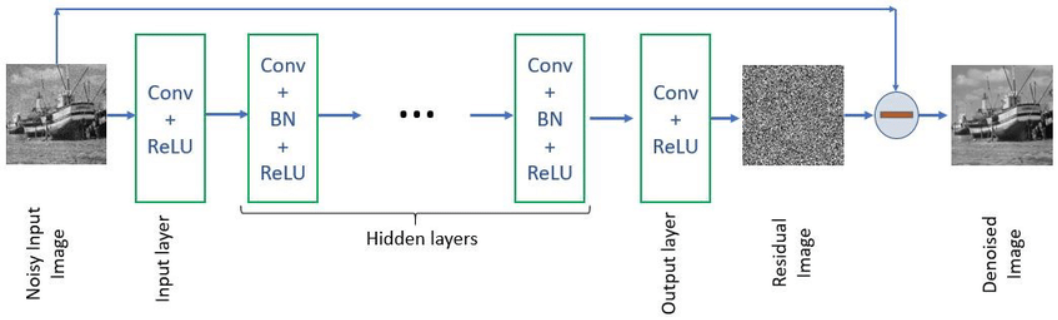
\includegraphics[angle=360,width=1.1\textwidth]{dncnn.png}\centering 
  \caption{FFDNet\cite{alawode2021dense}}
  \label{fig:resim_etiketi}
\end{figure}
\newpage

\section{Veri Setinin Oluşturulması}
\rule{\textwidth}{0.5pt}\\[10pt]

 \noindent Bu hafta, Pexels\cite{Pexels} ve Pixabay\cite{Pixabay} gibi web sitelerinden farklı türlerde toplam 100 görsel indirdim. Ardından bu görsellere 4 farklı gürültü ekleme algoritması uyguladım: Gauss gürültüsü, salt and pepper gürültüsü, Gauss and SP gürültüsü, ve Gauss bulanıklığı. Bu işlemlerin sonucunda toplamda 400 farklı çıktı elde ettim. Bu çıktılar sayesinde veri setimi oluşturmuş oldum. Görselleri indirmek için Pexels ve Pixabay gibi platformları tercih ettim çünkü bu siteler geniş bir görsel koleksiyonuna sahiptir ve farklı kategorilerde görsellere erişim sağlarlar. Bu çeşitlilik, veri setimin çeşitliliğini artırmama yardımcı oldu. Bu süreçte farklı gürültü türlerini anlamak ve bu gürültülerin görüntüler üzerindeki etkilerini gözlemlemek de önemli bir deneyim oldu.\vspace{0,5cm}

\noindent Ardından, her görsel üzerine farklı gürültü eklemek için 4 farklı algoritma kullandım:\vspace{0,5cm}

\noindent Gauss Gürültüsü: Bu algoritma\cite{Github}, pikseller üzerinde gauss dağılımına göre rastgele değerler ekler, böylece görselde yumuşak bir gürültü efekti oluşturur.\vspace{0,5cm}

\noindent Salt and Pepper Gürültüsü: Bu algoritma\cite{Github2}, piksellerin bazılarını siyah-beyaz veya beyaz-siyah olarak değiştirerek görselde noktasal bir gürültü oluşturur.\vspace{0,5cm}

\noindent Gauss and SP Gürültüsü: Bu algoritma, gauss ve salt-and-pepper gürültülerini birleştirir, böylece hem gauss gürültü hem de noktasal gürültü efekti elde edilir.\vspace{0,5cm}

\noindent Gauss Bulanıklığı: Bu algoritma\cite{OpenCV}, görselde bulanıklık yaratır ve keskin kenarları yumuşatır.\vspace{0,5cm}

%\section{Gauss Gürültüsü}
\begin{figure}
     \centering
 \noindent 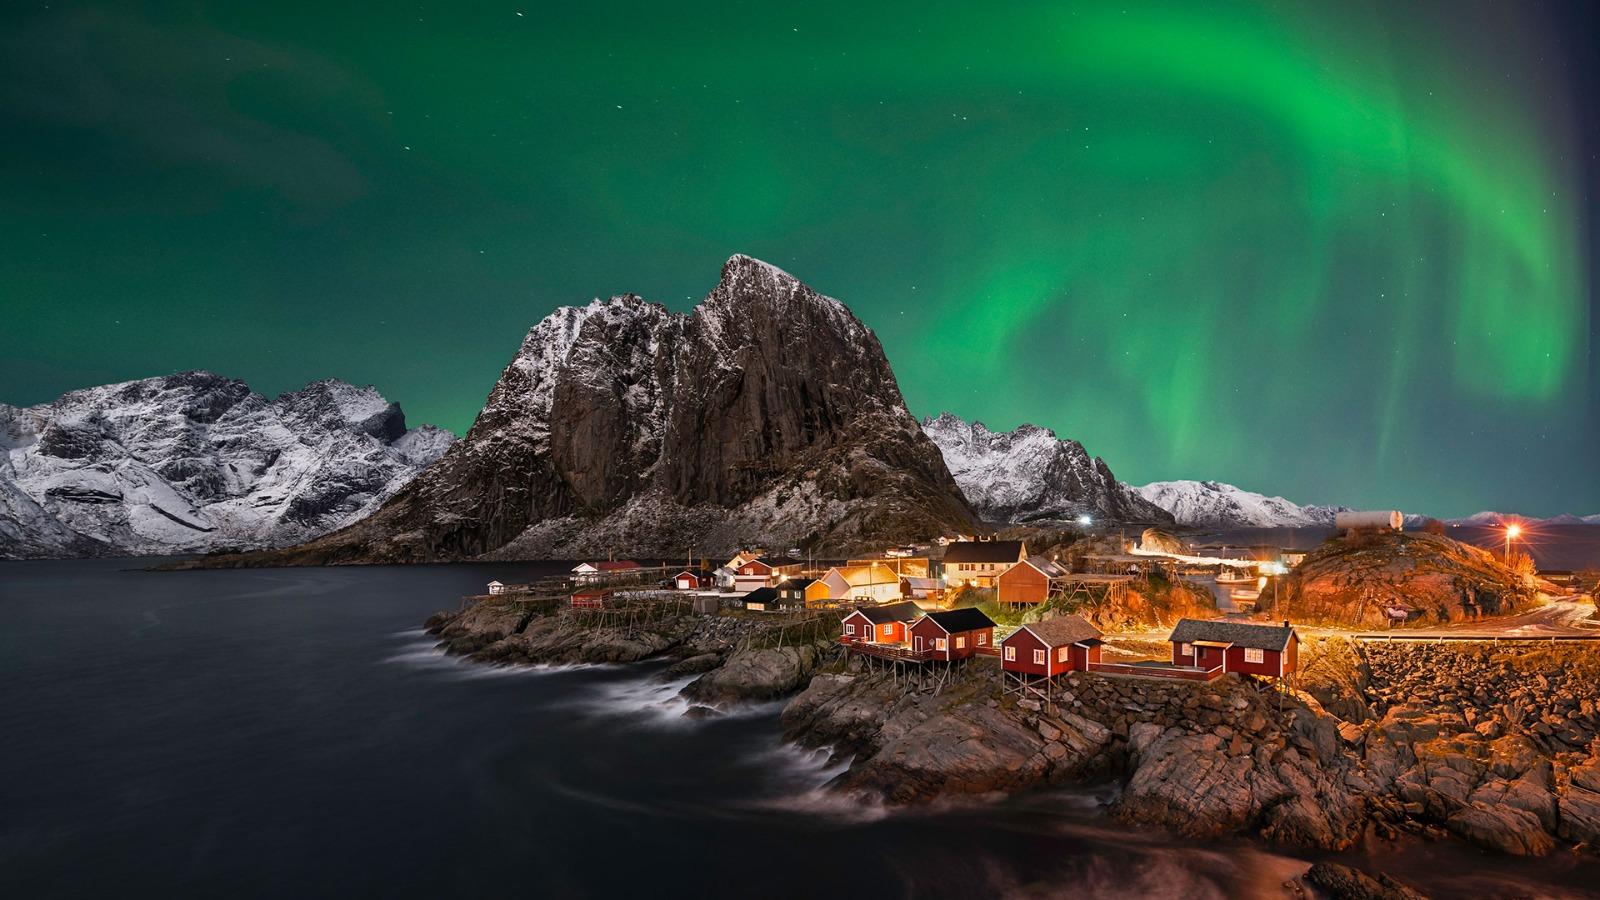
\includegraphics[angle=360,width=1.1\textwidth]{9.jpg}\centering 
  \caption{Orijinal Görsel}
  \label{fig:resim_etiketi}
\end{figure}

%\section{Gauss Gürültüsü}
\begin{figure}
     \centering
 \noindent 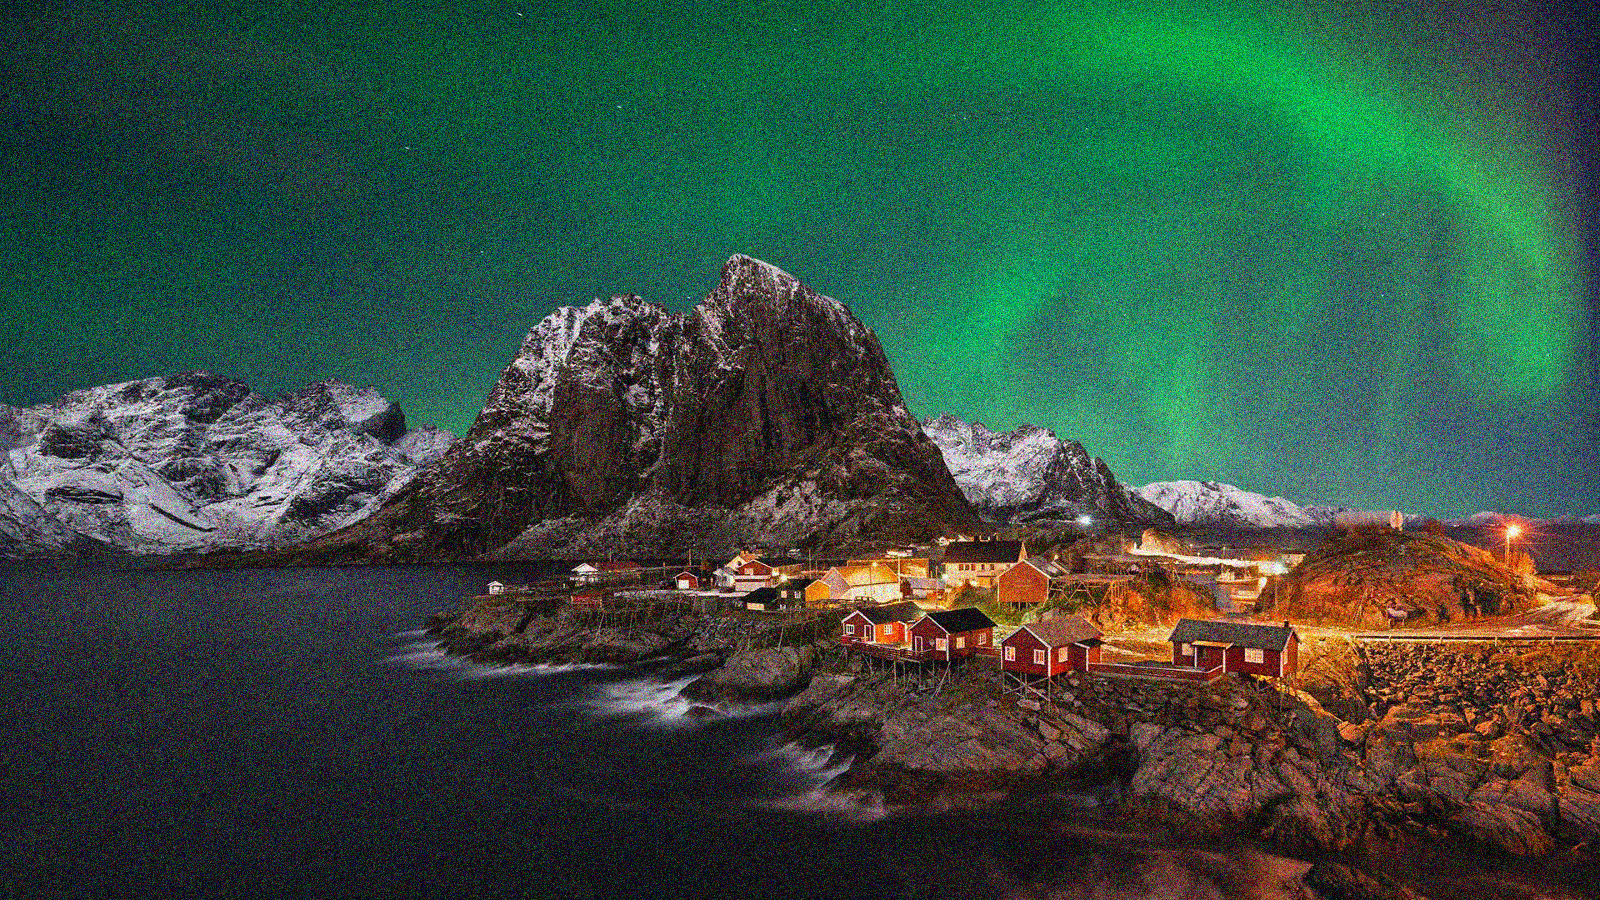
\includegraphics[angle=360,width=1.1\textwidth]{GaussN.png}\centering 
  \caption{Gauss Gürültüsü}
  \label{fig:resim_etiketi}
\end{figure}


%\section{Salt and Pepper Gürültüsü}
\begin{figure}
     \centering
  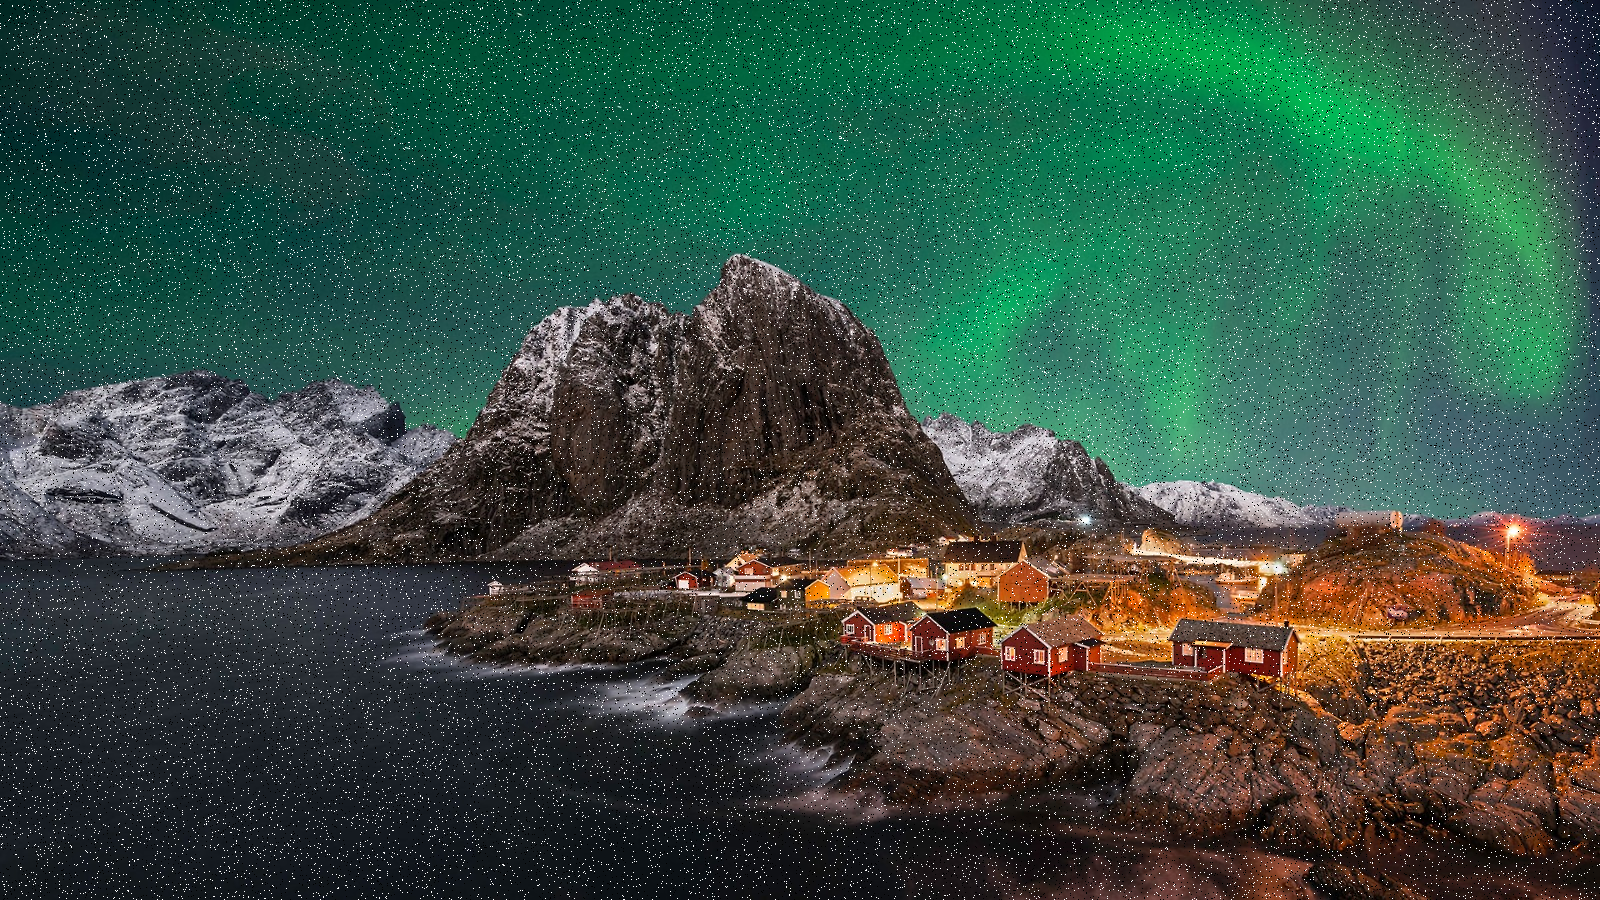
\includegraphics[angle=360,width=1.1\textwidth]{SPN.png}\centering 
  \caption{Salt and Pepper Gürültüsü}
  \label{fig:resim_etiketi}
\end{figure}

%\section{Gauss and SP Gürültüsü}
\begin{figure}
     \centering
  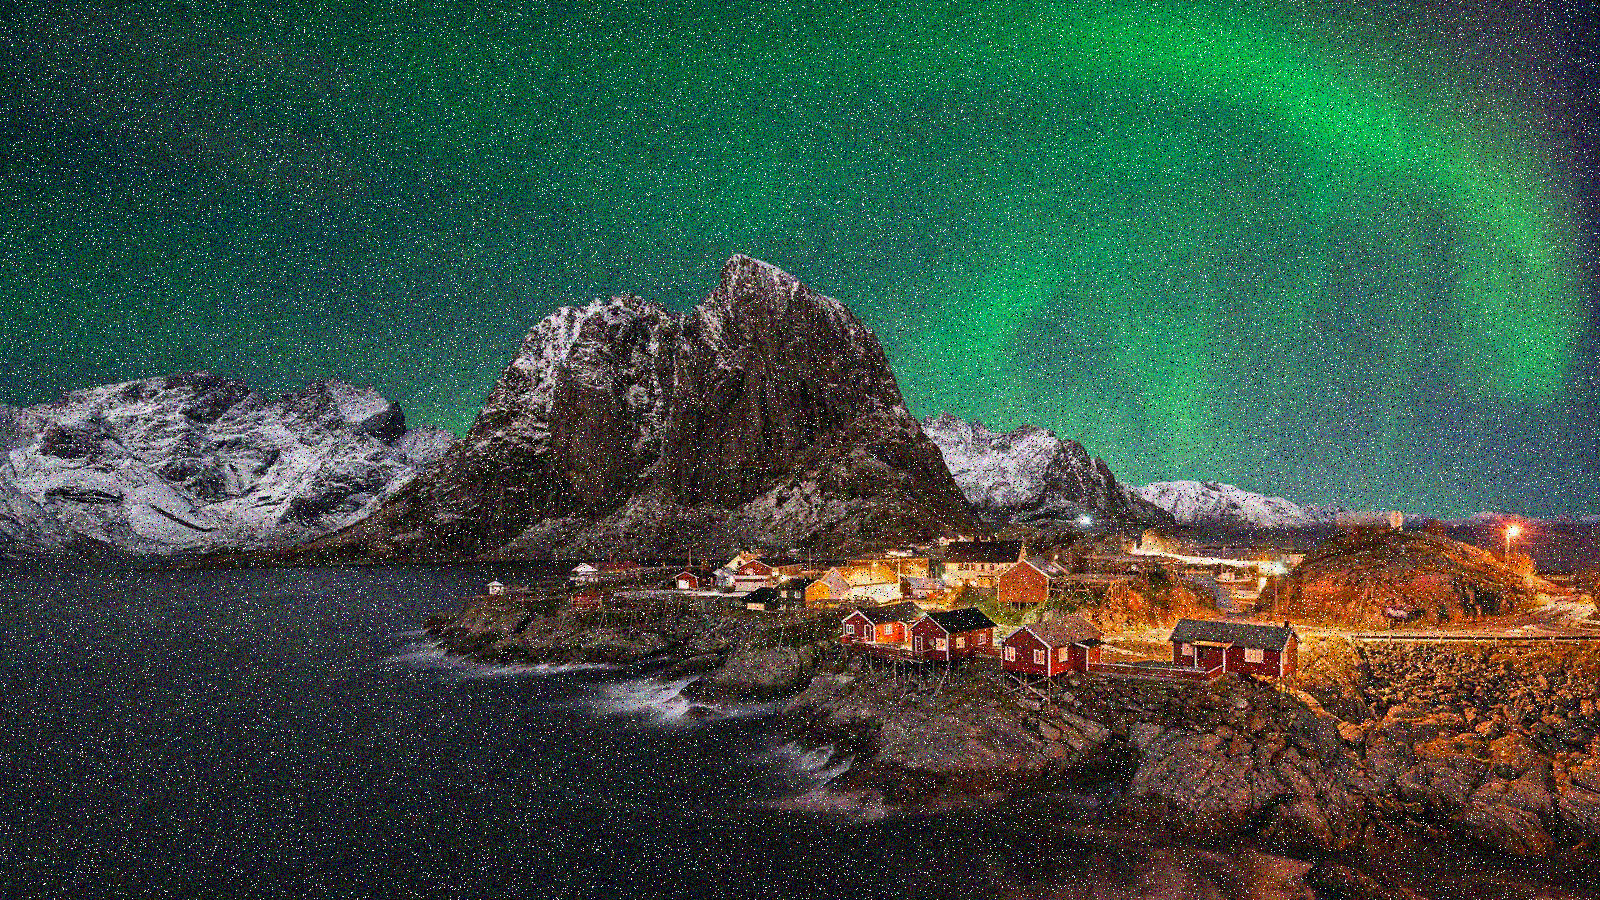
\includegraphics[angle=360,width=1.1\textwidth]{GaussAndSPN.png}\centering 
  \caption{Gauss and SP Gürültüsü}
  \label{fig:resim_etiketi}
\end{figure}

%\section{Gauss Bulanıklığı Gürültüsü}
\begin{figure}
     \centering
  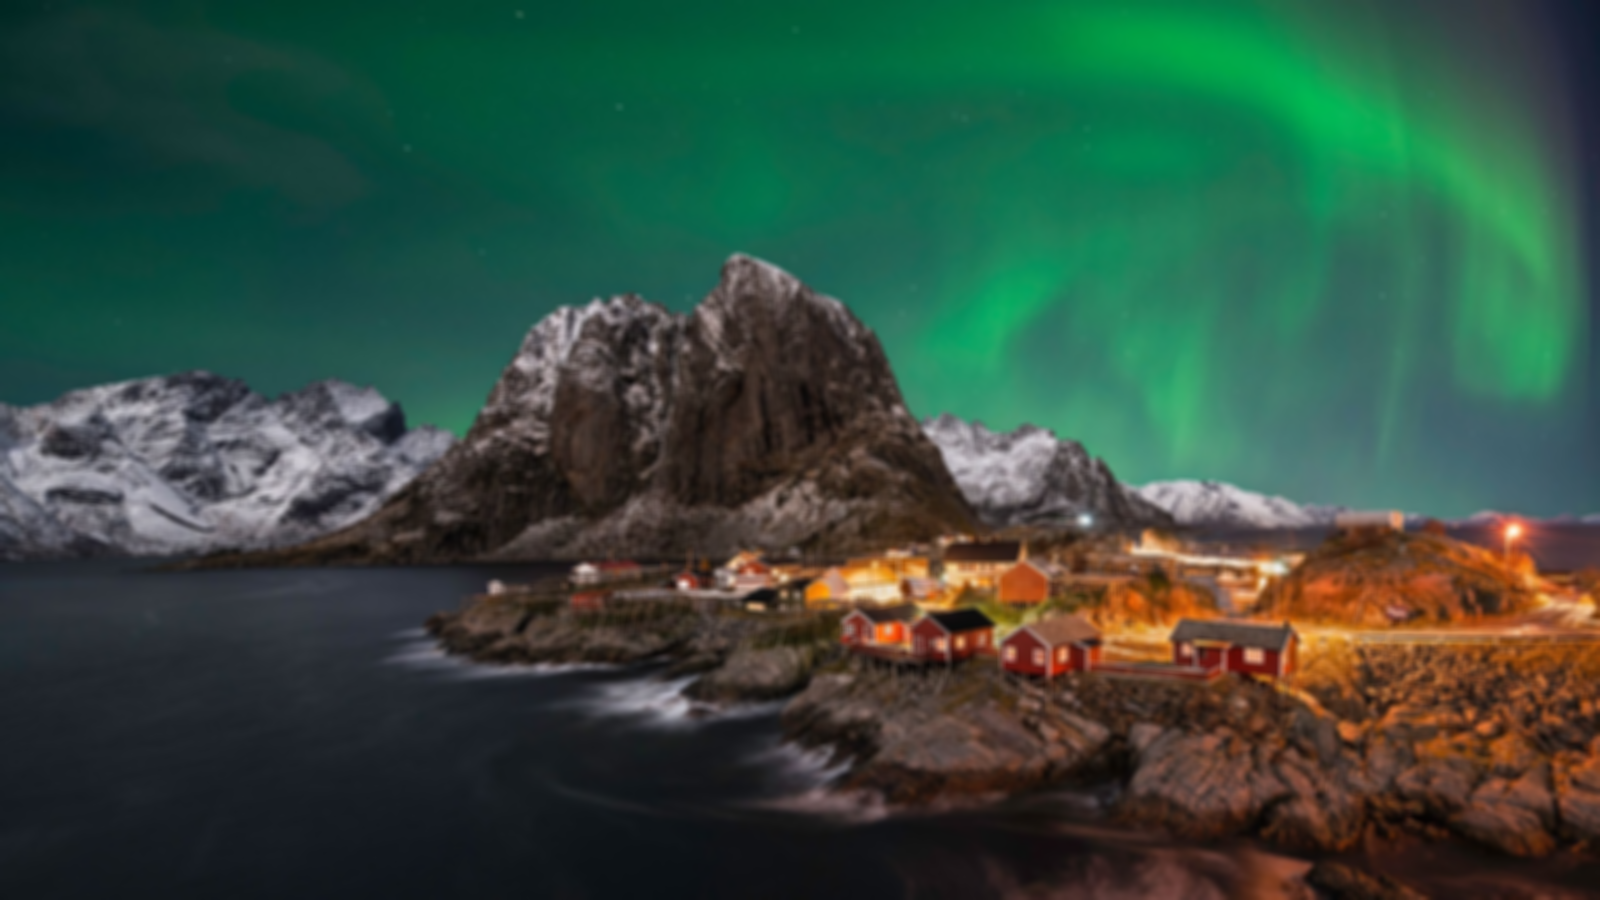
\includegraphics[angle=360,width=1.1\textwidth]{GaussBulanıklıgı.png}\centering 
  \caption{Gauss Bulanıklığı Gürültüsü}
  \label{fig:resim_etiketi}
\end{figure}

\newpage
\noindent Gösterdiğim algoritmaları kullanarak elde ettiğim görselleri gürültü türüne göre sınıflandırdım.\vspace{0,5cm}

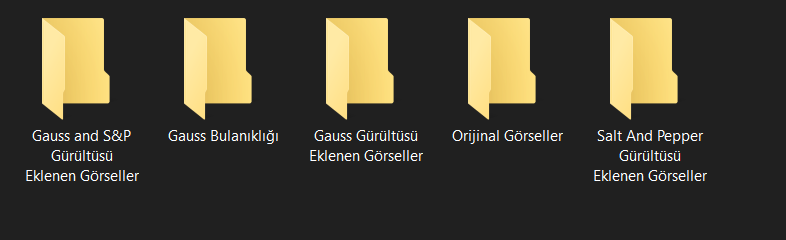
\includegraphics[width=1\textwidth]{Sınıflandırma.png}\vspace{0,5cm}

\newpage
\section{Yapay Zeka Oluşturulması}
\rule{\textwidth}{0.5pt}\\[10pt]

\noindent Bu hafta, bu projenin önceden yapılmış örneklerine\cite{Github3} bakarak yapacağım modelin nasıl yapılacağını, kodları anlayarak kendi projemde nelerin kullanılacağını ve kodlamamımı nasıl yapacağımı öğrenerek örnek projeler oluşturdum.\vspace{0.5cm}

\noindent Öncelikle yaptığım örnekler için hazır veri setleri kullandım. Bu örnekleri geliştirerek yapacağım asıl projede kendi veri setimi kullanacağım. Bu örneklerde hazır veri seti kullanmamın nedeni veri setindeki verilerin boyutunun aynı ve küçük olmasıdır. Böylece daha hızlı eğitimler yaparak kodların işlevselliğini hızlı bir şekilde kontrol edebilirim. Şu anki amacım kodları ve mantığını öğrenmek olduğu için örneklerimde bu veri setlerini kullandım.\vspace{0.5cm}

\noindent İlk oluşturduğum örnek için MNIST(Modified National Institute of Standards and Technology Database) veri setini kullandım. Bu veri seti 28x28 boyutunda, el yazısı rakamlardan oluşan siyah-beyaz bir veri setidir.\vspace{0.5cm}

\noindent İkinci oluşturduğum örnek için CIFAR-10(Canadian Institute For Advanced Research) veri setini kullandım. Bu veri seti 32x32 boyutunda gündelik hayattan pek çok görsel içeren,10 farklı sınıftan oluşan renkli bir veri setidir\vspace{0.5cm}

\noindent İki örneğin de kayıp fonksiyonlarıyla kayıp oranlarını grafikleştirdim. \vspace{0.5cm}

\renewcommand{\figurename}{Şekil}

\begin{figure}[htbp]
     \centering
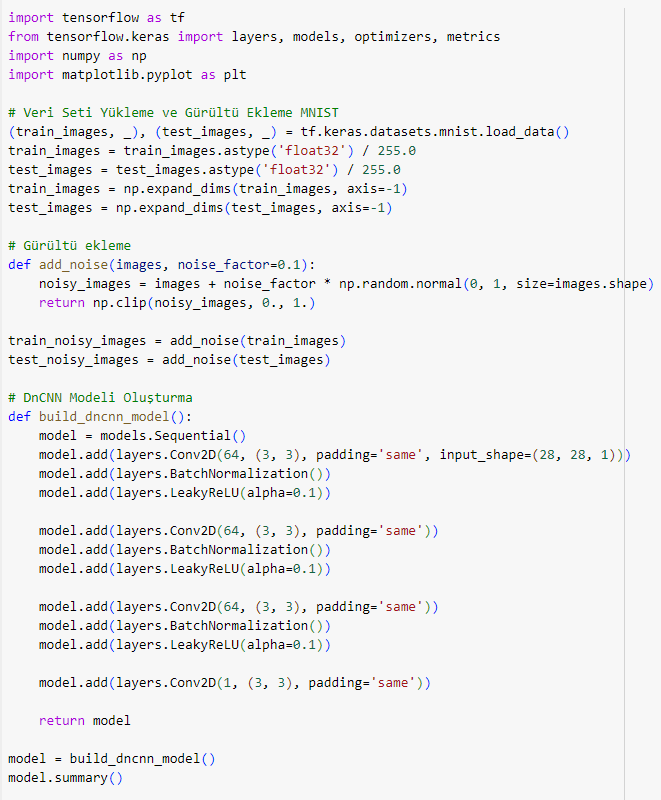
\includegraphics[angle=360,width=1.1\textwidth]{mnıst1.png}\centering 
  \caption{Kod}
  \label{fig:resim_etiketi}
\end{figure}

\renewcommand{\figurename}{Şekil}

\begin{figure}[htbp]
     \centering
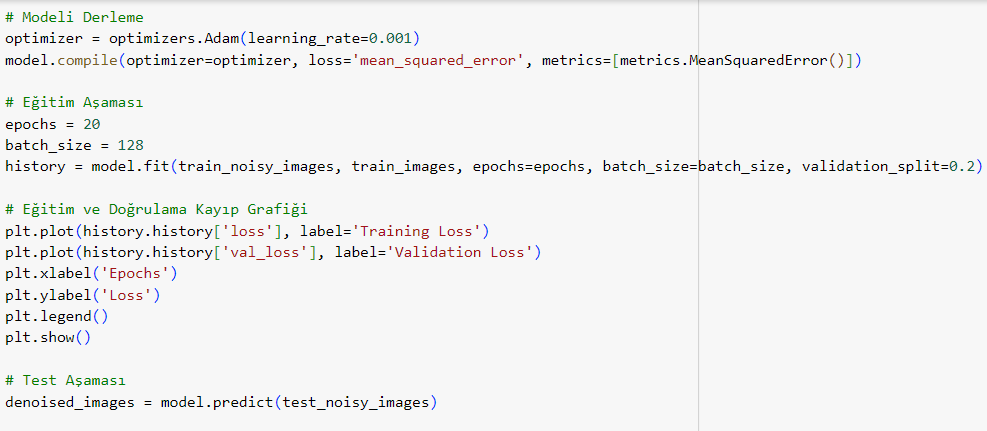
\includegraphics[angle=360,width=1.1\textwidth]{mnıst2.png}\centering 
  \caption{Kod}
  \label{fig:resim_etiketi}
\end{figure}

\renewcommand{\figurename}{Şekil}

\begin{figure}[htbp]
     \centering
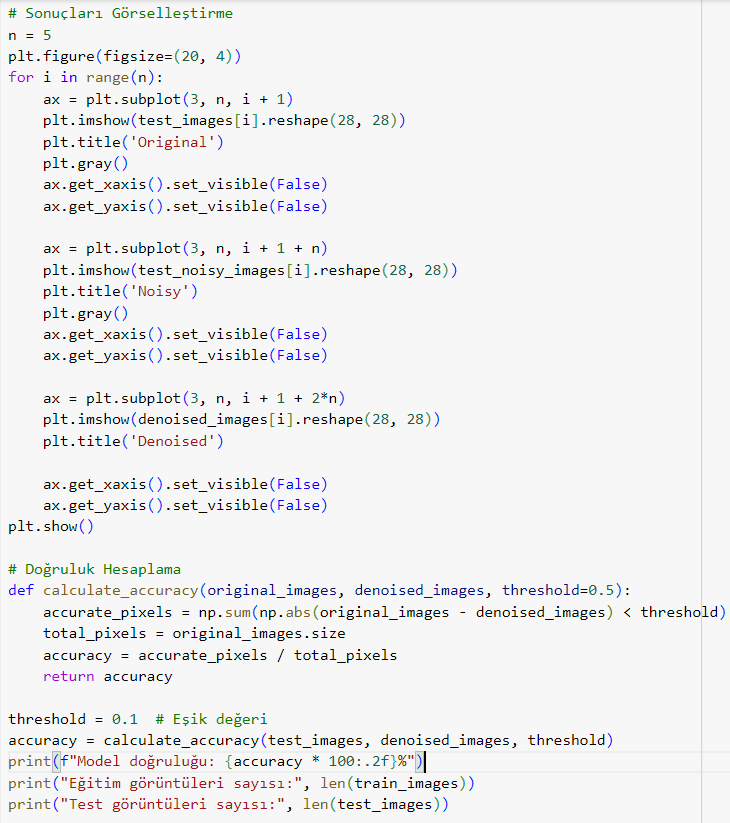
\includegraphics[angle=360,width=1.1\textwidth]{Mnıst3.png}\centering 
  \caption{Kod}
  \label{fig:resim_etiketi}
\end{figure}


\clearpage
\noindent Epoch sayılarına göre başarı oranları değişmektedir.

\renewcommand{\tablename}{Tablo}

\begin{table}[h!]
    \centering
    \resizebox{1\textwidth}{!}{
    \begin{tabular}{cc}
        \toprule
        \textbf{Epoch Sayısı} & \textbf{Doğruluk Oranı} \\ \midrule
        Epoch Sayısı 20 ise & 96.81 \\ 
        Epoch Sayısı 50 ise & 97.45 \\ 
        Epoch Sayısı 100 ise & 98.10 \\ \bottomrule
    \end{tabular}
    }
    \label{tab:ModelDoğrulukları}
    \caption{Epoch Sayısının Model Doğruluğu ile Bağlantısı}
\end{table}
\vspace{2cm}

\noindent İki örneğin de kayıp fonksiyonlarıyla kayıp oranlarını grafikleştirdim. \vspace{0.5cm}

\renewcommand{\figurename}{Şekil}

\begin{figure}[htbp]
     \centering
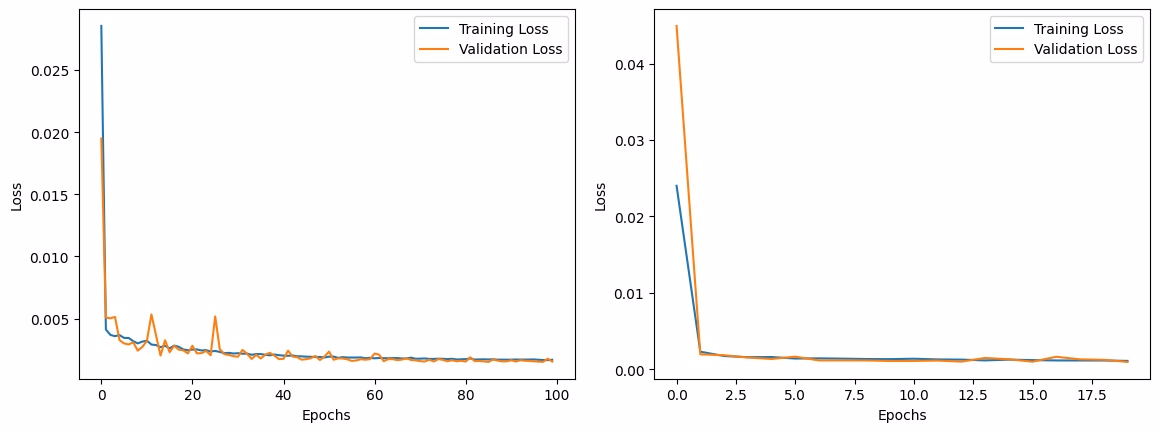
\includegraphics[angle=360,width=1\textwidth]{yz3(4).jpg}\centering 
  \caption{Kayıp Grafikleri}
  \label{fig:resim_etiketi}
\end{figure}

\clearpage

\noindent Burada yapmış olduğum 2 örneğin sonuçlarını göreceksiniz. \vspace{0.5 cm}


\begin{figure}[htbp]
     \centering
 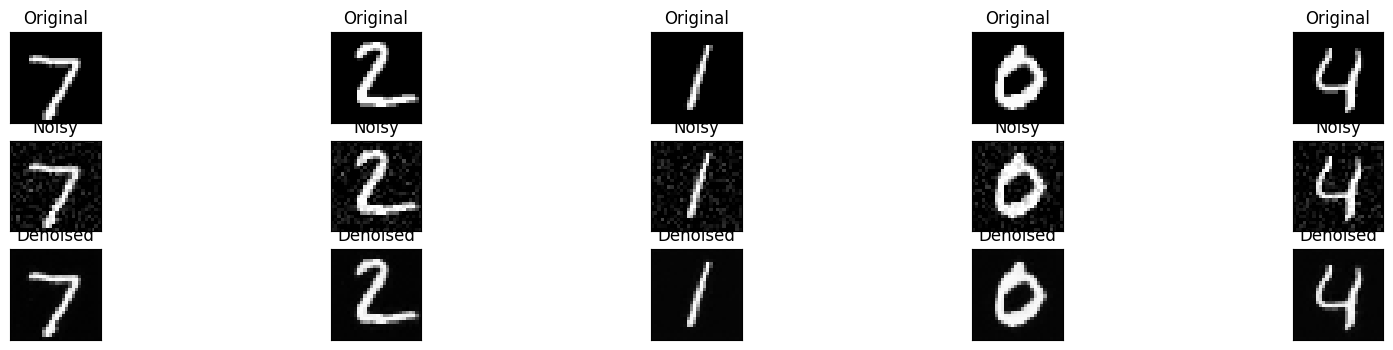
\includegraphics[angle=360,width=1\textwidth]{yz3.png}\centering 
  \caption{İlk Örneğin Sonucu}
  \label{fig:resim_etiketi}
\end{figure} \vspace{1 cm}


\begin{figure}[htbp]
     \centering
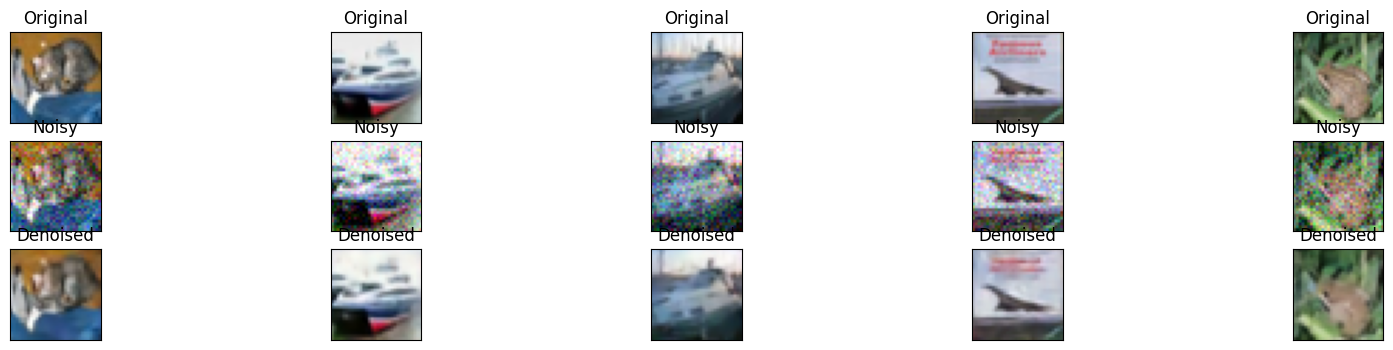
\includegraphics[angle=360,width=1\textwidth]{yz3(1).png}\centering 
  \caption{İkinci Örneğin Sonucu}
  \label{fig:resim_etiketi}
\end{figure}


\subsection{BatchNormalization Katmanının İşlevselliği}
\rule{\textwidth}{0.5pt}\\[10pt]

\noindent BatchNormalization katmanı, derin öğrenme modellerindeki eğitimi hızlandırmak ve daha iyi sonuçlar elde etmek için kullanılan bir tekniktir. Bu katman, her bir öğrenme döneminde mini toplu işlem yapılarak ağırlıkları ve önyargıları normalize eder. Bunu yaparak, ağırlıkların daha istikrarlı olmasını sağlar, aşırı uydurma (overfitting) riskini azaltır ve daha hızlı bir eğitim süreci sağlar.\vspace{0.5cm}

\noindent Örnek kodda zaten verileri [0,1] arasında normalize ediyordu ve modelin içinde yine de normalleştirme katmanları vardı ve bu durumun model için işlevselliğini test ettim. \vspace{0.5cm}

\noindent Modelin BatchNormalization katmanları var iken ve BatchNormalization katmanları çıkarıldıktan sonra modelin performansına nasıl etki ettiğine bakalım. \vspace{0.5cm}

\renewcommand{\tablename}{Tablo}

\begin{table}[h!]
    \centering
    \resizebox{1\textwidth}{!}{
    \begin{tabular}{cc}
        \toprule
        \textbf{BatchNormalization Katmanı} & \textbf{Doğruluk Oranı} \\ \midrule
        BN Katmanı varken & 97.70 \\ 
        BN Katmanı yokken & 98.28 \\ \bottomrule
    \end{tabular}
    }
    \label{tab:ModelDoğrulukları}
    \caption{BatchNormalization Katmanının Etkisi}
\end{table}

\noindent Normalde BatchNormalization katmanı modelin doğruluğunu arttırmak için etkilidir ama bazı basit modellerde  bu katmanın varlığı doğruluğu düşürebilir. BatchNormalization katmanları ekstra bir karmaşıklık katmanıdır ve modelin karmaşıklığını artırır.\vspace{0.5cm}


\subsection{LeakyReLU ve ReLU Katmanları}
\rule{\textwidth}{0.5pt}\\[10pt]

\noindent ReLU\cite{Baeldung}, negatif girişlerde doğrusal olarak sıfırı alır. Yani, negatif bir değeri alırsa, çıkışı direkt olarak sıfır olur. Bu, modelin daha hızlı öğrenmesine ve daha az hesaplama maliyetine sahip olmasına yardımcı olabilir. Ancak, büyük negatif değerlerde sıfıra yakın çıkışlar alındığında, bu "ölü nöron" sorununa yol açabilir. Ölü nöronlar, eğitim sırasında hiçbir bilgiyi iletemeyen veya güncellemeyen nöronlardır. \vspace{0.5cm}

\noindent LeakyReLU\cite{Baeldung}, negatif girişlerde de bir miktar eğim sağlar. Yani, negatif bir değeri alırsa, çıkışı sıfırdan küçük olur ancak tam olarak sıfır değil. Bu, modelin daha büyük negatif değerlerle de çalışmasına izin verir ve ölü nöron problemini azaltabilir. Alpha parametresi, bu eğimin ne kadar olacağını belirler; yani, negatif bölgedeki eğimin büyüklüğünü kontrol eder. \vspace{0.5cm}

\renewcommand{\figurename}{Şekil}

\begin{figure}[htbp]
     \centering
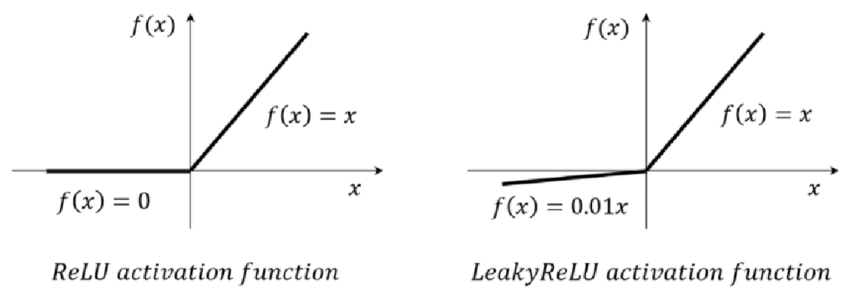
\includegraphics[angle=360,width=1\textwidth]{ReLU-activation-function-vs-LeakyReLU-activation-function.png}\centering 
  \caption{LeakyReLU ve ReLU \cite{Relu}}
  \label{fig:resim_etiketi}
\end{figure}

\clearpage
\noindent LeakyReLU'nun kullanılması, özellikle büyük veri setleri veya derin modellerle çalışırken ölü nöron sorununu azaltmaya yardımcı olabilir. Ancak, kullanılacak aktivasyon fonksiyonu modelin doğası ve veri setine bağlı olarak değişebilir. Bazı durumlarda, ReLU yeterli olabilirken, diğer durumlarda LeakyReLU daha iyi sonuçlar verebilir. 

\noindent Modelde ReLU ve LeakyReLU kullanınca modelin performansına nasıl etki ettiğine bakalım. \vspace{0.5cm}

\renewcommand{\tablename}{Tablo}

\begin{table}[h!]
    \centering
    \resizebox{1\textwidth}{!}{
    \begin{tabular}{cc}
        \toprule
        \textbf{ReLU ve LeakyReLU} & \textbf{Doğruluk Oranı} \\ \midrule
        ReLU & 98.27 \\ 
        LeakyRelu & 98.28 \\ \bottomrule
    \end{tabular}
    }
    \label{tab:ModelDoğrulukları}
    \caption{ReLU ve LeakyReLU Katmanlarının Etkisi}
\end{table}

\subsection{Modeli Kendi Veri Setime Uygulama}
\rule{\textwidth}{0.5pt}\\[10pt]

\noindent Kendi veri setimdeki görsellerin boyutlları büyük ve farklı olduğundan tüm görsellerin boyutlarını eşitliyorum. Örnek olarak boyutllarını (32,32,3) boyutunda eşitlersem modelin performansıyla ,(512,512,3) boyutunda eşitlersem modelin performansı arasında fark oluyor.

\renewcommand{\tablename}{Tablo}

\begin{table}[h!]
    \centering
    \resizebox{1\textwidth}{!}{
    \begin{tabular}{cc}
        \toprule
        \textbf{Görsel Boyutu } & \textbf{Doğruluk Oranı} \\ \midrule
        (32,32,3) iken & 91.20 \\ 
        (512,512,3) iken & 97.20 \\ \bottomrule
    \end{tabular}
    }
    \label{tab:ModelDoğrulukları}
    \caption{Görsel Boyutunun Etkisi}
\end{table}

\newpage
\noindent Conv2D katmanı yani evrişim katmanında filtre sayısını değiştirdiğimiz zaman modelin performansını etkiliyor.


\renewcommand{\tablename}{Tablo}

\begin{table}[h!]
    \centering
    \resizebox{1\textwidth}{!}{
    \begin{tabular}{cc}
        \toprule
        \textbf{Filtre sayısı  } & \textbf{Doğruluk Oranı} \\ \midrule
        (64) iken & 91.20 \\ 
        (128) iken & 92.37 \\ \bottomrule
    \end{tabular}
    }
    \label{tab:ModelDoğrulukları}
    \caption{Conv2D katmanındaki filtre sayısının Etkisi}
\end{table}

\noindent  NOT: Yapılmış olan performans değerlendirmeleri ve karşılaştırmaları kendi içinde olup diğer değerlendirmelerle bağlantılı değildir.

\subsection{PReLU Katmanı }
\rule{\textwidth}{0.5pt}\\[10pt]

\noindent Bu aktivasyon fonksiyonu, geleneksel ReLU'dan farklı olarak negatif girişler için öğrenilebilir bir eğim kullanır.\\[10pt]

\renewcommand{\figurename}{Şekil}
\begin{figure}[htbp]
     \centering
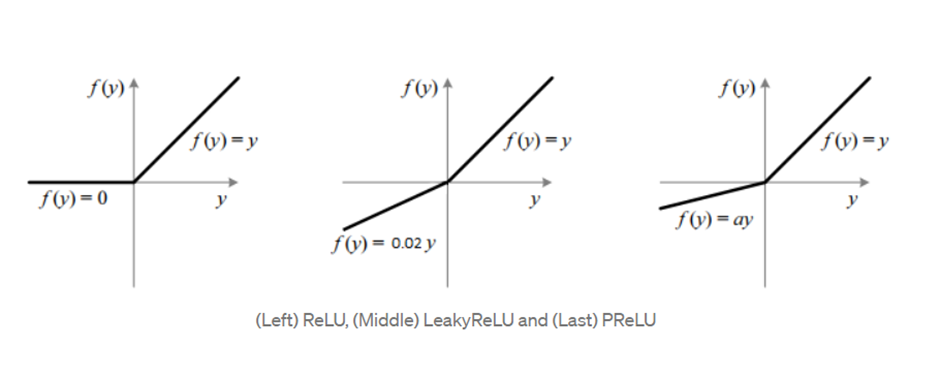
\includegraphics[angle=360,width=1.1\textwidth]{prelu.png}\centering 
  \caption{ReLU, LeakyReLU, PReLU\cite{Nomidl}}
  \label{fig:resim_etiketi}
\end{figure}

\noindent Burada a parametresi, negatif girişler için kullanılacak olan eğimi temsil eder. Bu eğim değeri, eğitim sırasında öğrenilen bir parametredir, yani model tarafından veriye uygun olarak ayarlanır.\\[10pt]

\subsection{Gürültü Türlerine Göre Model Performansı}
\rule{\textwidth}{0.5pt}\\[10pt]

\noindent Gaussian gürültü\cite{Wikipedia}, her piksel değerine normal dağılım ile belirlenen rastgele değerler ekleyen bir gürültü türüdür. \\[10pt]

\noindent Salt and pepper gürültüsü\cite{Wikipedia}, görüntüde rastgele piksellerin beyaz veya siyah olarak değiştirilmesi ile oluşur. \\[10pt]


\noindent Speckle gürültüsü\cite{Wikipedia2}, özellikle radar, tıbbi ultrason ve lazer görüntüleme sistemleri gibi koherent dalga tabanlı görüntüleme sistemlerinde görülür. Bu tür gürültü, görüntünün her pikselinin gerçek değerinin bir rastgele fraktal (kendine benzer) yapı tarafından çarpılması sonucu oluşur. \\[10pt]

\noindent Poisson gürültüsü (ya da foton gürültüsü)\cite{Wikipedia}, özellikle düşük ışıklı ortamlarda veya az sayıda foton sayımı içeren görüntüleme sistemlerinde yaygın olarak görülür.  \\[10pt]

\noindent Periodic gürültüsü\cite{Wikipedia}, görüntülerde düzenli ve tekrarlanan desenler şeklinde ortaya çıkan bir tür gürültüdür. Genellikle, dijital görüntüleme veya tarama cihazlarının mekanik titreşimleri veya elektriksel girişimlerinden kaynaklanır. \\[10pt]

\renewcommand{\tablename}{Tablo}

\begin{table}[h!]
    \centering
    \resizebox{1\textwidth}{!}{
    \begin{tabular}{cc}
        \toprule
        \textbf{Gürültü Türleri  } & \textbf{Doğruluk Oranı} \\ \midrule
        Salt and Paper Gürültüsü & 99.03 \\ 
        Gauss Bulanıklığı & 98.31 \\
        SP, Gauss Gürültüleri Beraber & 95.49 \\
        Speckle Noise & 99.87 \\ 
        Poisson Noise & 99.97 \\ 
        Periodic Noise & 99.98 \\ \bottomrule
    \end{tabular}
    }
    \label{tab:ModelDoğrulukları}
    \caption{Gürültü Türlerinin Etkisi}
\end{table}

\newpage
\noindent Bu doğruluk oranlarından anlaşılacağı üzere tek başına Salt and Paper gürültüsü çok karmaşık bir gürültü türü değil ve başarı oranı bayâ yüksek oluyor. Tek başına Gauss Bulanıklığı yine pek karmaşık bir gürültü türü değil ve bunun başarı oranı da yüksek. Son olarak iki tür beraber kullanıldığı zaman başarı oranı azımsanmayacak ölçüde düşüyor yani en karmaşık gürültü şekli beraber kullanıldıkları zaman oluyor.


\subsection{Veri Setini Kod İle İndirme ve Kullanma}
\rule{\textwidth}{0.5pt}\\[10pt]

\noindent Veri setini kod yardımı ile indirmek diğer türlü uğraşmaktan çok daha kolay. Görsellerin indireleceği web sitesine kaydolup oradan görsellere erişebilmek için API anahtarını kullanmak gerekiyor.\\[10pt]


\renewcommand{\figurename}{Şekil}
\begin{figure}[htbp]
     \centering
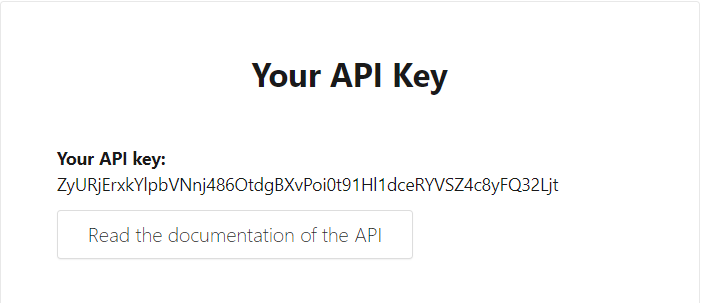
\includegraphics[angle=360,width=0.8\textwidth]{apıpexels.png}\centering 
  \caption{Pexels API \cite{API}}
  \label{fig:resim_etiketi}
\end{figure}


\noindent Örnek kodlardan yardım alarak\cite{geeksforgeeks} yazdığım buradaki kod Apı anahtarını kullanarak websitesinden belirtilen kategoride ve sayıda görsel indirmeye yarıyor.\\[10pt]

\renewcommand{\figurename}{Şekil}
\begin{figure}[htbp]
     \centering
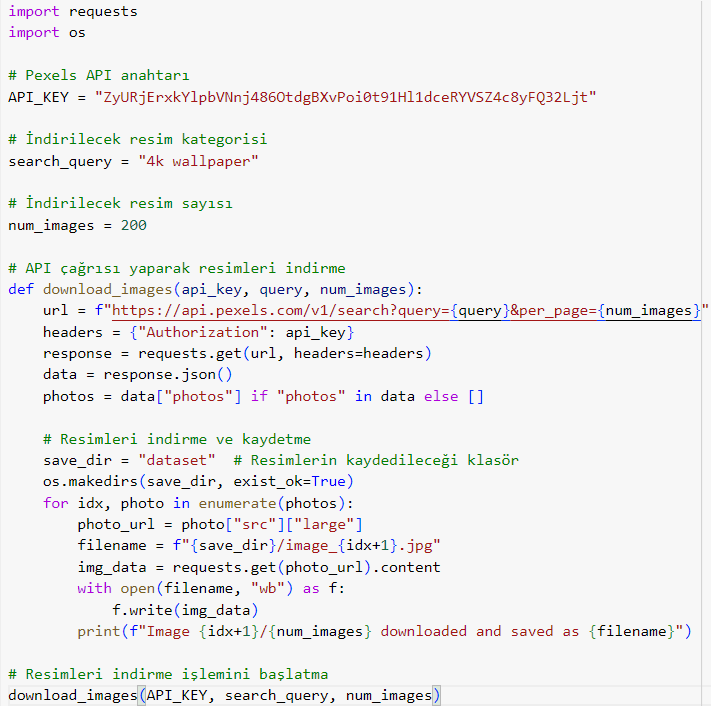
\includegraphics[angle=360,width=1.1\textwidth]{ApıKod.png}\centering 
  \caption{Kod}
  \label{fig:resim_etiketi}
\end{figure}

\clearpage
\subsection{Yüksek Boyutlu Görsellerde Model Performansı}
\rule{\textwidth}{0.5pt}\\[10pt]


\noindent Büyük boyutlu görsellerle eğitim yapıldığı zaman modelin performansı düşüyor. Örneğin Gaussian and Salt-and-Pepper Gürültüsü küçük boyutlu veri setiyle eğitildiği zaman model doğrulu daha yüksek. \\[10pt]

\noindent Büyük boyutlu görsellerle eğitilen modelde Gaussian Gürültüsü kullanınca model performansı 98.19, Gaussian and Salt-and-Pepper Gürültüsü kullanınca 93.61 oldu.  \\[10pt]

\noindent Modelin Doğrululuğunu arttırmak için ekstra Conv2D ve LeakyReLU katmanları eklendi ama artış beklenirken düşüş yaşandı yani işe yaramadı. \\[10pt]

\noindent Bunların temeldeki sebebi büyük görsellerin eğitim için boyutunun asıl boyutlarından daha küçük bir boyuta indirgenmesi. Boyut indirgenince piksel sayısı azalıyor ve örneğin normalde 4 piksel olan bir alanı 1 piksele indirgeniyor.\\[10pt]

\noindent Modelin Doğrululuğunu arttırmak için farklı ReLU katmanları denendi ama en iyi performansı LeakyReLU verdi.\\[10pt]

\noindent Modelin performansının artmasını sağlayan şeyler, deneyerek uygun epoch ve batch size değerlerinin bulunması oldu. Bu iyileştirmelerden sonra modelin doğruluğu 95.94 oldu.\\[10pt]


\noindent Büyük boyuttaki görsellerin bir sorunu da çok fazla GPU Ram'i kullanmalarıdır. ReLU katmanları arasında deneme yaparken ReLU katmanı kullanırken GPU yetersiz hatası verdi. Kullanılan oturumun GPU Ram'i 22.5GB'dı ve 40GB GPU Ram'ine sahip oturuma geçildiği zaman kod çalıştı. \\[10pt]

\newpage
\subsection{Test Görseli}
\rule{\textwidth}{0.5pt}\\[10pt]

\noindent Test görselinin veri setinden değil başka bir yerden alınıp test edilmesi. Böylece modelin başka gürültülü görselleri de başarılı şekilde gürültüsüz haline getirdiğini görüyoruz.\\[10pt]

\renewcommand{\figurename}{Şekil}
\begin{figure}[htbp]
     \centering
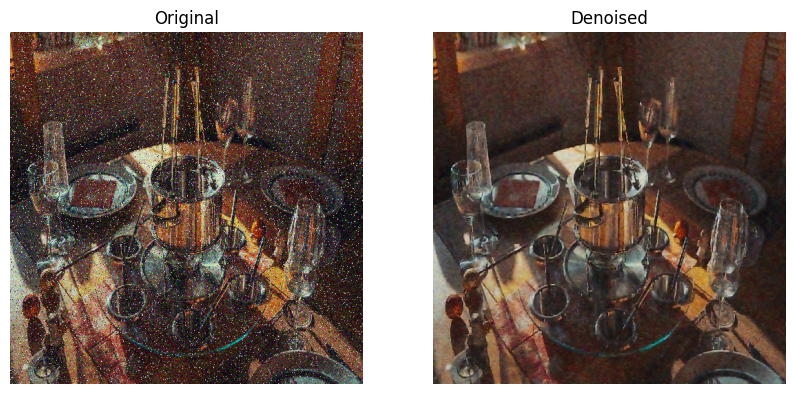
\includegraphics[angle=360,width=1.1\textwidth]{test.png}\centering 
  \caption{Test Görseli\cite{Pexels}}
  \label{fig:resim_etiketi}
\end{figure}

\subsection{Görsel Boyutunun Modelle Bağlantısı}
\rule{\textwidth}{0.5pt}\\[10pt]

\noindent Veri setindeki görsellerin boyutu yüksek olduğu zaman boyut düşürülmesi yapıldı çünkü işlem yükünden dolayı büyük boyutlu görsellerle eğitim yapmak daha zordur. Ve boyut düşürüldüğü zaman kod düzgün bir şekilde çalışıyor.\\[10pt]

\noindent Aynı şekilde veri setindeki görsellerin boyutu düşük olduğunda yükseltilip eğitim yapıldığı zaman model doğruluğu 99.99 oluyor ve aslında düzgün bir şekilde gürültüleri gideremiyor. \\[10pt] 

\renewcommand{\figurename}{Şekil}
\begin{figure}[htbp]
     \centering
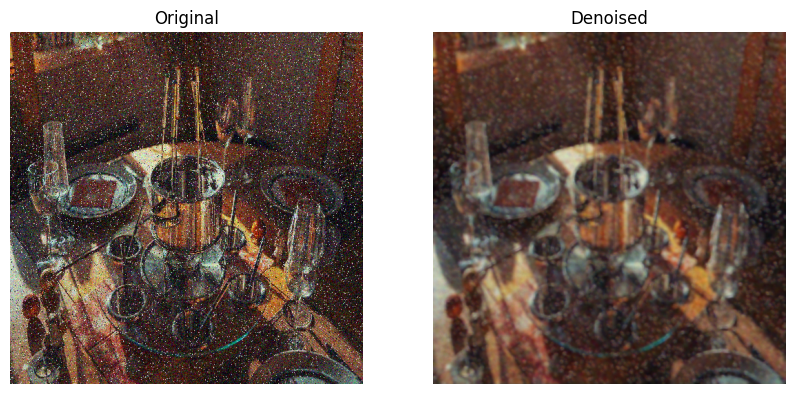
\includegraphics[angle=360,width=1.1\textwidth]{boyutDüşürme.png}\centering 
  \caption{Veri Seti Boyutu Yükseltildiği Zaman Test Görüntüsü }
  \label{fig:resim_etiketi}
\end{figure}

\noindent Bu durumu düzeltmek ve gürültüleri gidermek için değişikler yapılsa da işe yaramadı ve düzgün bir şekilde gürültüler giderilemedi. \\[10pt]


\subsection{Görüntü Kalitesi }
\rule{\textwidth}{0.5pt}\\[10pt]

\noindent PSNR (Peak Signal-to-Noise Ratio)\cite{Wikipedia3}, dijital görüntü işleme ve sinyal işleme alanlarında kullanılan bir kalite ölçütüdür. PSNR, iki görüntü arasındaki benzerliği ölçer ve genellikle bir referans görüntü ile bozulmuş veya sıkıştırılmış bir görüntü arasındaki farkı değerlendirmek için kullanılır. PSNR değeri, desibel (dB) cinsinden ifade edilir. \\[10pt]

\noindent PSNR, temel olarak ortalama kare hatasını (Mean Squared Error, MSE) kullanarak hesaplanır. MSE, iki görüntü arasındaki piksel farklarının karelerinin ortalamasını alır. PSNR, bu MSE değerini kullanarak hesaplanır ve şu formüle sahiptir: \\[3pt]

PSNR (Peak Signal-to-Noise Ratio)
\begin{equation}
    \text{PSNR} = 20 \cdot \log_{10}\left(\frac{\text{MAX}_I}{\sqrt{\text{MSE}}}\right)
\end{equation} \\[3pt]


\noindent MAX I görüntüdeki maksimum piksel değeridir. Genellikle 8-bit görüntüler için bu değer 255'tir.\\[3pt]

\noindent PSNR'nin yüksek bir değeri, iki görüntü arasındaki farkın az olduğunu ve dolayısıyla görüntü kalitesinin yüksek olduğunu gösterir. \\[3pt]

\renewcommand{\figurename}{Şekil}
\begin{figure}[htbp]
     \centering
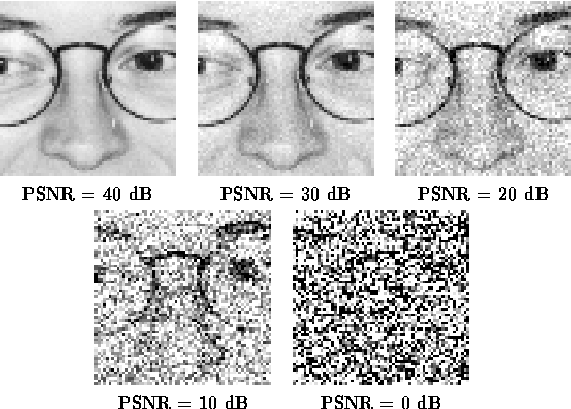
\includegraphics[angle=360,width=0.7\textwidth]{Illustration-of-the-PSNR-measure.png}\centering 
  \caption{PSNR\cite{sohag2013novel}}
  \label{fig:resim_etiketi}
\end{figure}


\noindent SSIM (Structural Similarity Index)\cite{Wikipedia4}, iki görüntü arasındaki benzerliği ölçmek için kullanılan bir metrikdir. SSIM görüntülerin yapısal bilgilerini dikkate alarak daha insan algısına uygun bir kalite değerlendirmesi sağlar.\\[3pt]

\noindent SSIM, üç ana bileşeni karşılaştırarak hesaplanır: parlaklık, kontrast ve yapı. Bu bileşenler, insan gözünün görüntüleri nasıl algıladığını daha iyi yansıtır.
SSIM formülü şu şekildedir: \\[3pt]

SSIM (Structural Similarity Index)
\begin{equation}
    \text{SSIM}(x, y) = \frac{(2\mu_x \mu_y + C_1)(2\sigma_{xy} + C_2)}{(\mu_x^2 + \mu_y^2 + C_1)(\sigma_x^2 + \sigma_y^2 + C_2)}
\end{equation} \\[3pt]

\noindent SSIM değeri -1 ile 1 arasında değişir. Değer 1'e ne kadar yakınsa, iki görüntü arasındaki benzerlik o kadar yüksektir. \\[3pt]

\clearpage
\renewcommand{\figurename}{Şekil}
\begin{figure}[htbp]
     \centering
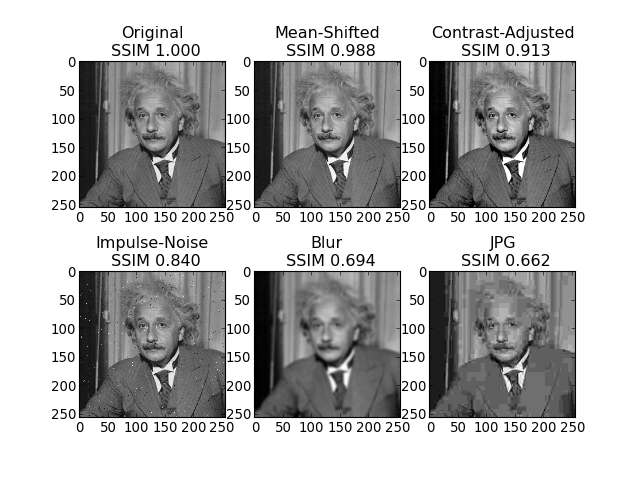
\includegraphics[angle=360,width=1\textwidth]{ssim-1.png}\centering 
  \caption{SSIM\cite{SSIM}}
  \label{fig:resim_etiketi}
\end{figure}


\section{Sonuç}

\noindent Bu raporda sunulan yapay zeka projesi, görüntülerdeki gürültüleri etkin bir şekilde gidermeyi amaçlayan bir modelin geliştirilmesi ve değerlendirilmesini kapsamaktadır. Yapılan deneyler ve sonuçlar, modelimizin bu amaca ulaşmada yüksek bir doğruluk ve verimlilik sağladığını göstermiştir. Farklı epoch sayılarında yapılan eğitimler sonucunda modelimizin performansının önemli ölçüde arttığı gözlemlenmiştir. \\[3pt]

\noindent Sonuç olarak, geliştirilen yapay zeka modelinin, görüntülerin kalitesini artırmada ve gürültüleri başarıyla gidermede başarılı bir şekilde çalıştığı belirlenmiştir. Bu çalışma, gelecekte daha büyük veri setleri ve farklı gürültü türleri üzerinde yapılacak iyileştirmelerle daha da geliştirilebilir. Elde edilen bu başarı, görüntü işleme alanında yapay zeka kullanımının ne kadar etkili ve potansiyel dolu olduğunu bir kez daha ortaya koymaktadır.  \\[3pt]

\clearpage
\newpage

\bibliographystyle{ieeetr}
\bibliography{ref8}

\end{document}